\documentclass{beamer}
\usetheme{Madrid}
\usepackage{graphicx}
\usepackage{booktabs}
\usepackage{amsmath}
\usepackage{hyperref}
\usepackage{listings}
\usepackage{xcolor}
\usepackage{appendixnumberbeamer} % Damit das \appendix einen eigenen Zähler hat

\AtBeginSection[]{
  \begin{frame}
    \centering
    \Huge\insertsection
  \end{frame}
}

\lstset{
  language=Python,
  basicstyle=\ttfamily\small,
  keywordstyle=\color{blue},
  commentstyle=\color{gray},
  stringstyle=\color{red},
  numbers=left,
  numberstyle=\tiny\color{gray},
  stepnumber=1,
  numbersep=5pt,
  tabsize=1,
  showspaces=false,
  showstringspaces=false,
  breaklines=true
}

\title[Glom Segmentation]{Glomerulus Segmentation in Kidney Biopsies}
\subtitle{Computer Vision Project, Group 9}
\author[Group 9]{Lukas Göbl, Peer Schäfer, Lukas Scheib}
\date{15.07.2025}



\begin{document}

\begin{frame}
    \titlepage
\end{frame}

% Problem statement
\begin{frame}{Problem Statement}
    \textbf{General:} Accurate segmentation of glomeruli in kidney biopsy images is crucial for diagnosing chronic kidney diseases.

    \vspace{0.5cm}

    \textbf{Precise Tasks:} Segment glomeruli at patch-level and whole-slide level in kidney tissue images as part of the MICCAI 2024 KPIs Challenge.
\end{frame}

\begin{frame}{WSI Example: train\textbackslash56Nx\textbackslash12\_116}
    % Full sized WSI
    % Challenge: Whole-slide images (WSIs) are large, up to 80k pixels in size.
    \begin{figure}
        \vspace{-0.14cm}
        \centering
        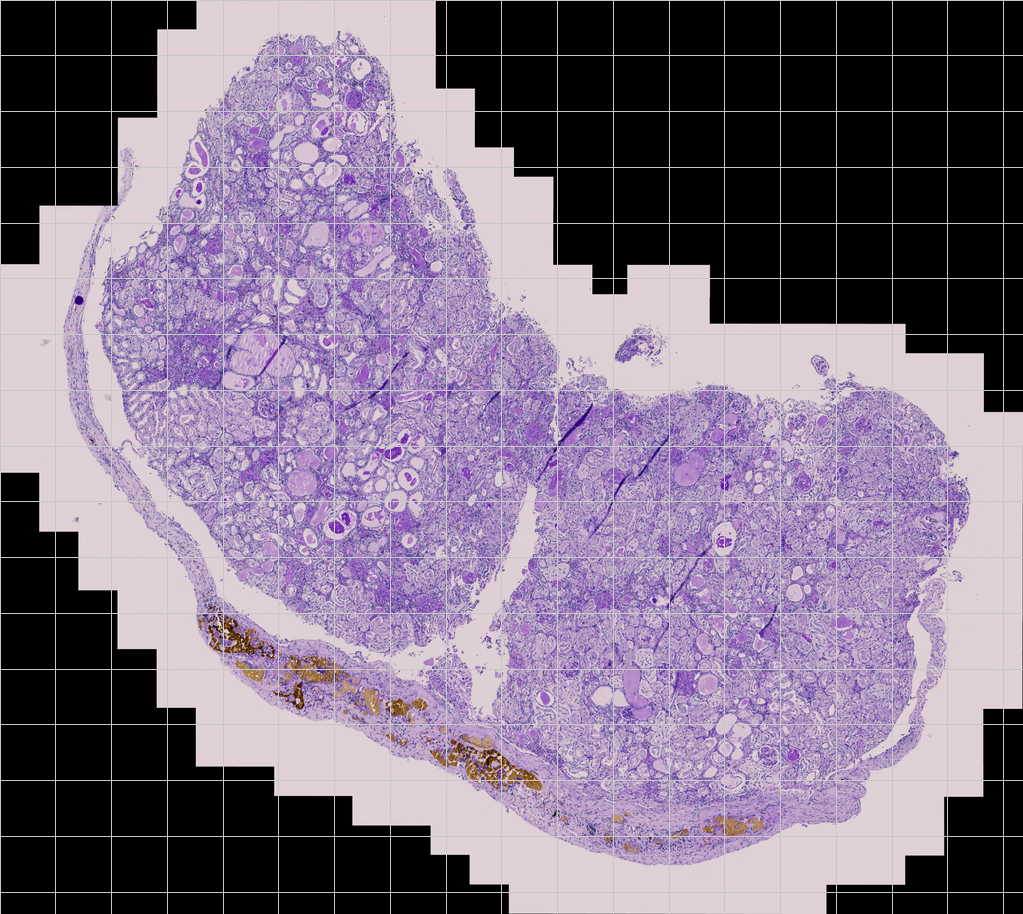
\includegraphics[height=0.877\textheight]{Images/wsi_thumbnail_with_grid.png}
    \end{figure}
\end{frame}

\begin{frame}{WSI Mask Example: train\textbackslash56Nx\textbackslash12\_116}
    %Challenge: Small fraction of pixels are glomeruli $\rightarrow$ models tend to predict background.
    % Dataset: WSIs and WSIs as patched images and their masks, highly imbalanced (background:glomeruli $\approx$ 23:1).
    \begin{figure}
        \vspace{-0.14cm}
        \centering
        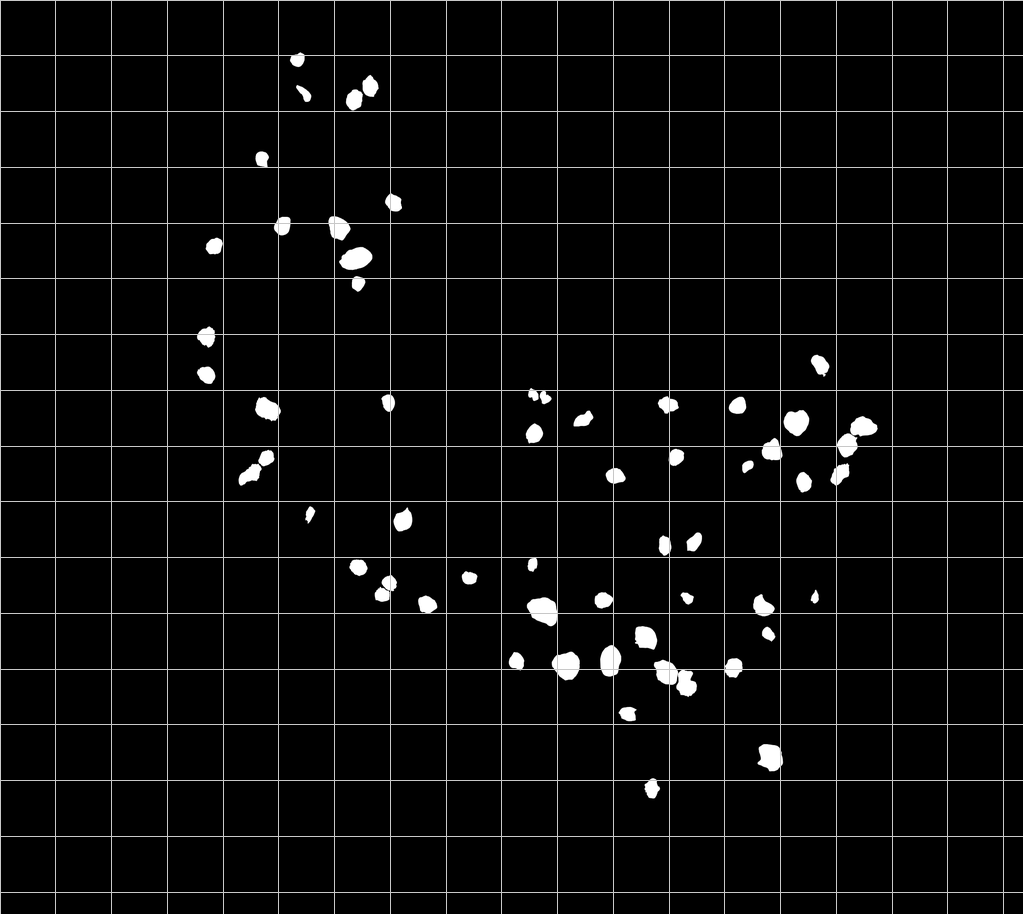
\includegraphics[height=0.877\textheight]{Images/mask_thumbnail_with_grid.png}
    \end{figure}

\end{frame}

% Methods and motivation
\begin{frame}{VariableUNet Model}
    \begin{itemize}
        \item Standard UNet architecture with 8 double convolution layers split into encoder and decoder layers with skip connections between them.
        \item Dilated convolutions in the bottleneck (with dilation rates 1, 2, 4 on $\frac{1}{3}$ of the channels each) for multi-scale feature extraction.\footnote{\href{https://doi.org/10.1117/1.JMI.8.6.067501}{Li et al. (2021)}}
        \item Channel quantities scale with variable patch size.
    \end{itemize}
    
        
\end{frame}

% Experimental design
\begin{frame}{Experimental Design}
    \begin{itemize}
        \item Trained on official KPIs dataset (train/val/test splits).
        \item Combined binary cross entropy (BCE) and Dice loss to address class imbalance. 
        \item Hyperparameter tuning: BCE/Dice ratio, Dice smooth, positive class weighting for BCE, learning rate for Adam optimizer.
        \item Experiments with different patch sizes ($256^2$ and $2048^2$ pixels) and data subsets.
        \item Evaluated using accuracy, precision, recall, and $F_1$-score.
        \item Qualitative assessment via visual inspection.
    \end{itemize}
\end{frame}

% Results
\begin{frame}{Metrics of our best performing Models}
    % After lot of testing _v2
    % Important: 256 patch size tested on 256 test set, 2048 patch size tested on 2048 test set.
    % 256px preds should be scaled up before testing
    \begin{table}[t]
        \centering
        \begin{tabular}{c|c|cccc}
            \toprule
            Patch size & Split & Accuracy & Precision & Recall & $F_1$-score \\
            \midrule
            256 & Validation & 0.9781 & 0.7479 & 0.7660 & 0.7569 \\
            & Test       & 0.9757 & 0.7537 & 0.7133 & 0.7330 \\
            \midrule
            2048 & Validation & 0.9705 & 0.9299 & 0.3662 & 0.5255 \\
            & Test       & 0.9643 & 0.9159 & 0.2616 & 0.4070 \\
            \bottomrule
        \end{tabular}
    \end{table}
    \begin{block}{Hyperparameters:}
        \begin{itemize}
            \item BCEDiceLoss Ratio = 0.8
            \item BCE Positive Weight = 25
            \item Dice Smooth = $10^{-6}$
            \item Learning Rate = $10^{-4}$
        \end{itemize}
    \end{block}
\end{frame}

% Experimental design
\begin{frame}{WSI Segmentation}
    % Optional second task UwU
    \textbf{Implemented patching pipeline with the following hyperparameters:}
    \begin{itemize}
        \item Patch size
        \item Patch overlap (stride)
        \item Trivial patch threshold for positive pixels
    \end{itemize}

    \vspace{0.5cm}

    \textbf{Possible next steps:}
    \begin{itemize}
        \item Implementation of a stitching pipeline to combine patch predictions into a full WSI mask.
        \item Train VariableUNet using the complete patching and stitching pipeline.
    \end{itemize}
\end{frame}

% Discussion
\begin{frame}{Discussion}
    \textbf{What worked:}
    \begin{itemize}
        \item BCE + Dice loss crucial for recall and $F_1$-score.
        \item Hyperparameter tuning improved glom detection.
        \item WSIs can be patched for patch-level segmentation.
    \end{itemize}

    \vspace{0.5cm}

    \textbf{Limitations:}
    \begin{itemize}
        \item Instability in training, especially with full-size patches.
        \item Our configurations, trained on small patches, did not generalize well to larger patches.
        \item No empirical validation on WSI segmentation due to time constraints.
    \end{itemize}
\end{frame}

% Discussion
\begin{frame}{Discussion}
    \textbf{In retrospect:}
    \begin{itemize}
        \item Greater emphasis on pre- and post-processing (downsampling patches and upsampling predictions).
        \item More in-depth data exploration regarding samples of different diseases.
    \end{itemize}

    \vspace{0.5cm}

    \textbf{Future work:}
    \begin{itemize}
        \item Exploring different model architectures and methods.
        \item Search for more robust hyperparameters and domain adaptation.
        \item Continued work on WSI segmentation pipeline.
    \end{itemize}
\end{frame}

\begin{frame}{Example Model Prediction}
    \begin{figure}
        \centering
        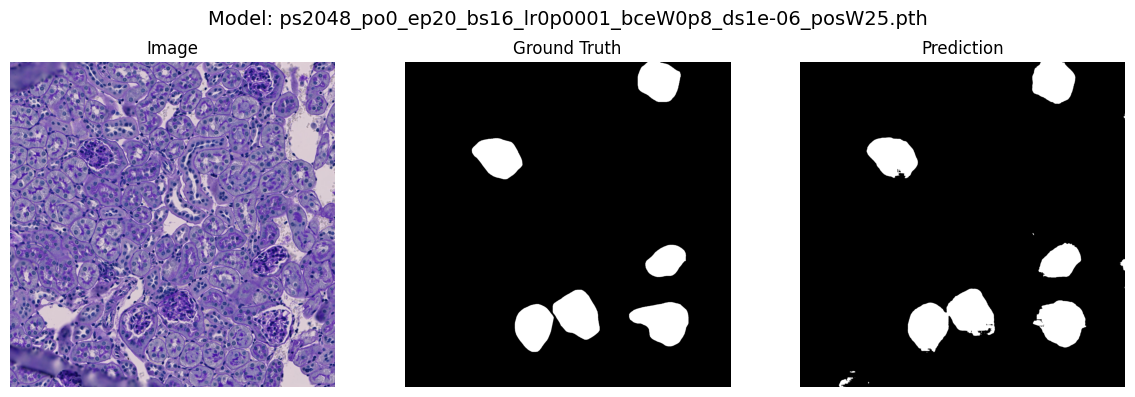
\includegraphics[width=\textwidth]{Images/big_good.png}
    \end{figure}
\end{frame}

\appendix

% Appendix
\section{Backup}

% Dilated bottleneck
\begin{frame}{UNet Architecture}
    \begin{figure}
        \centering
        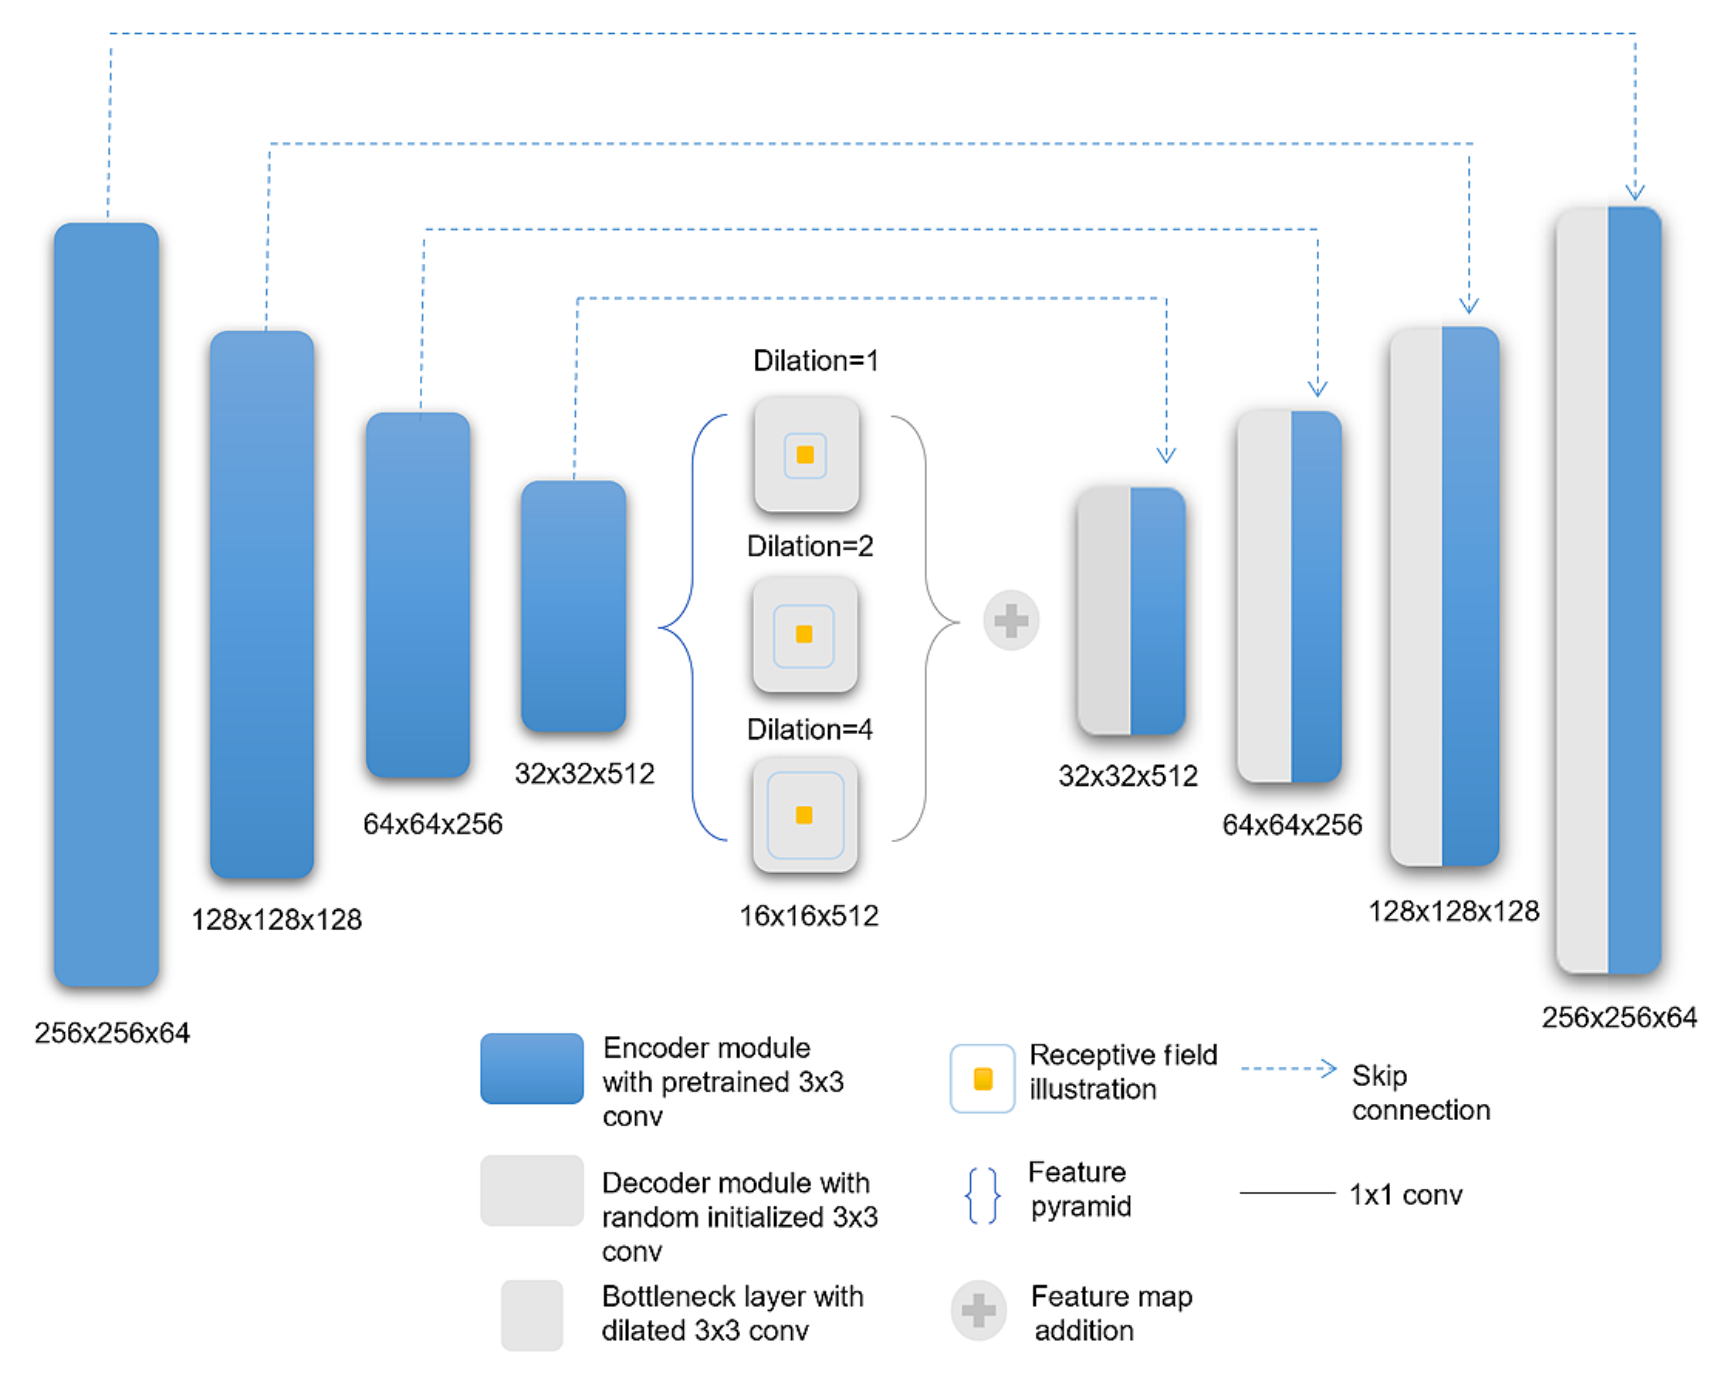
\includegraphics[height=0.7\textheight]{Images/UNetArchitecture.png}
        \caption{Source: \href{https://doi.org/10.1117/1.JMI.8.6.067501}{Li et al. (2021)}, Figure 3 (edited)}
    \end{figure}
\end{frame}

% Double Convolution
\begin{frame}[fragile]{Double Convolution in our Code Base}
    \begin{lstlisting}[language=Python]
class DoubleConv(nn.Module):
    def __init__(self, in_channels, out_channels):
        super().__init__()
        self.double_conv = nn.Sequential(
            nn.Conv2d(in_channels, out_channels, 3, padding=1),
            nn.BatchNorm2d(out_channels),
            nn.ReLU(inplace=True),
            nn.Conv2d(out_channels, out_channels, 3, padding=1),
            nn.BatchNorm2d(out_channels),
            nn.ReLU(inplace=True),
        )

    def forward(self, x):
        return self.double_conv(x)
    \end{lstlisting}
\end{frame}

% Heat Map
\begin{frame}{$F_1$-Score Heat Map from Experiment 2}
    \begin{figure}
        \centering
        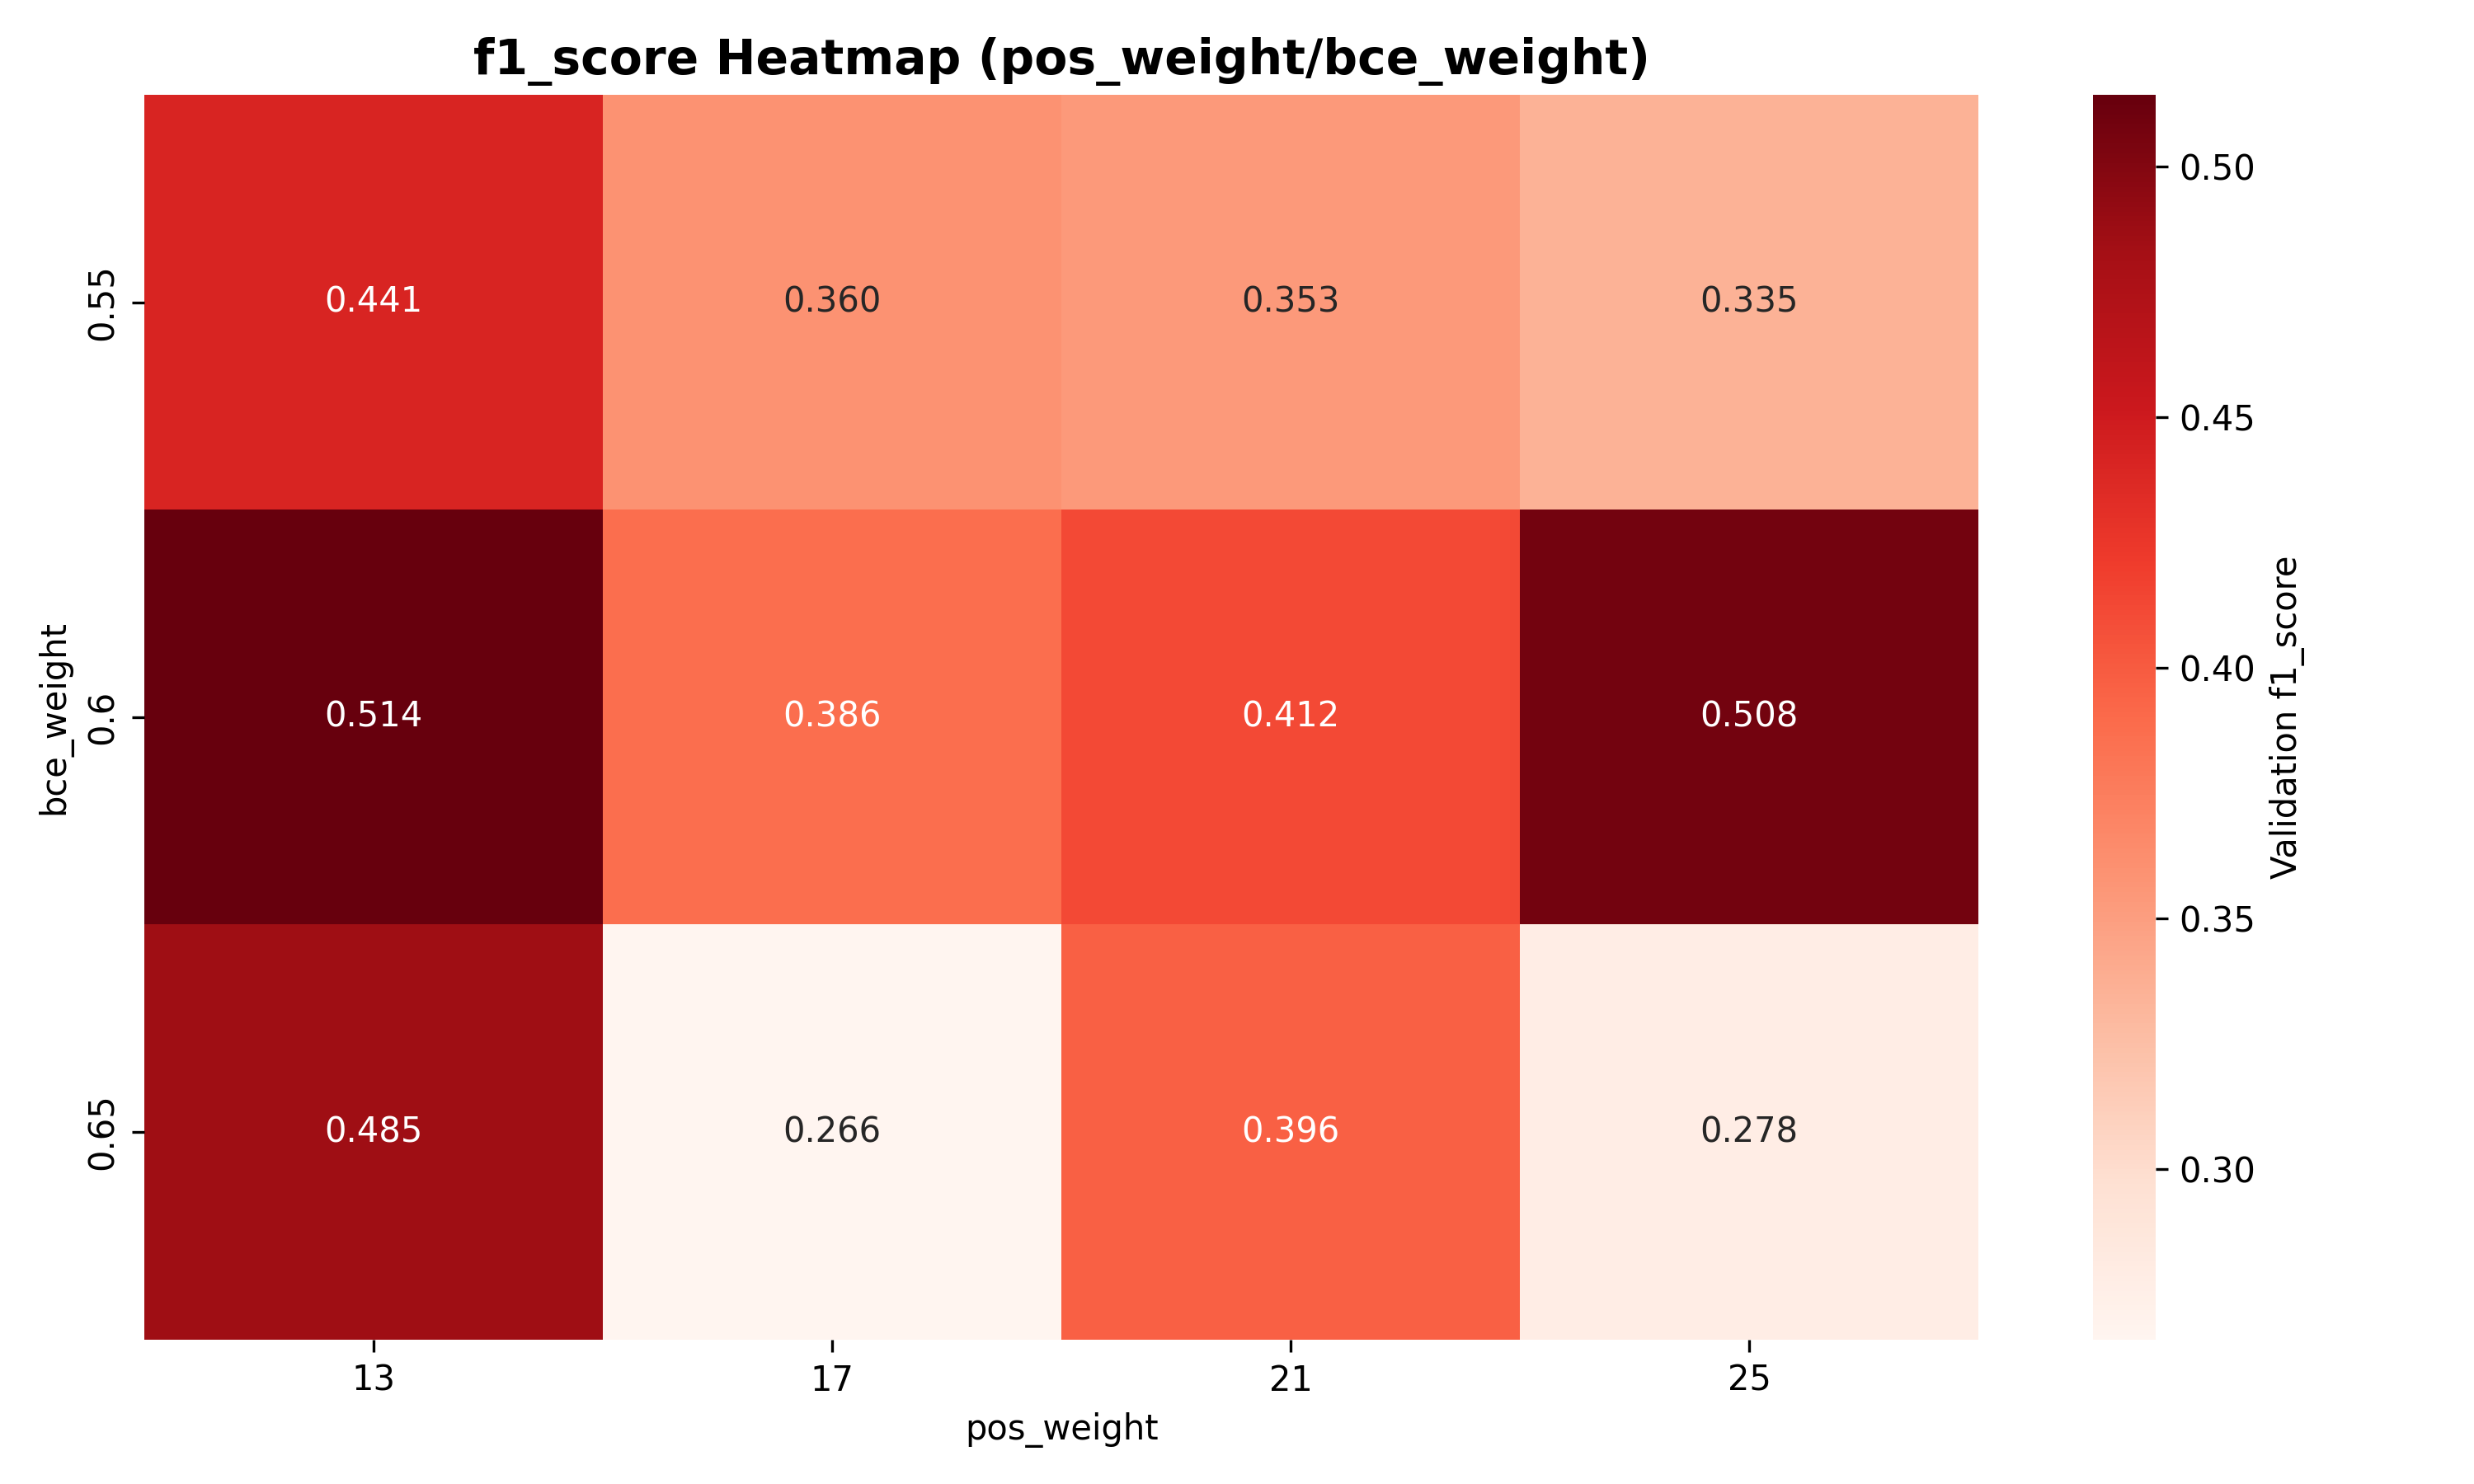
\includegraphics[height=0.7\textheight]{Images/12_heatmap_f1_score_by_weights.png}
    \end{figure}
\end{frame}

% Heat Map
\begin{frame}{Recall Heat Map from Experiment 2}
    \begin{figure}
        \centering
        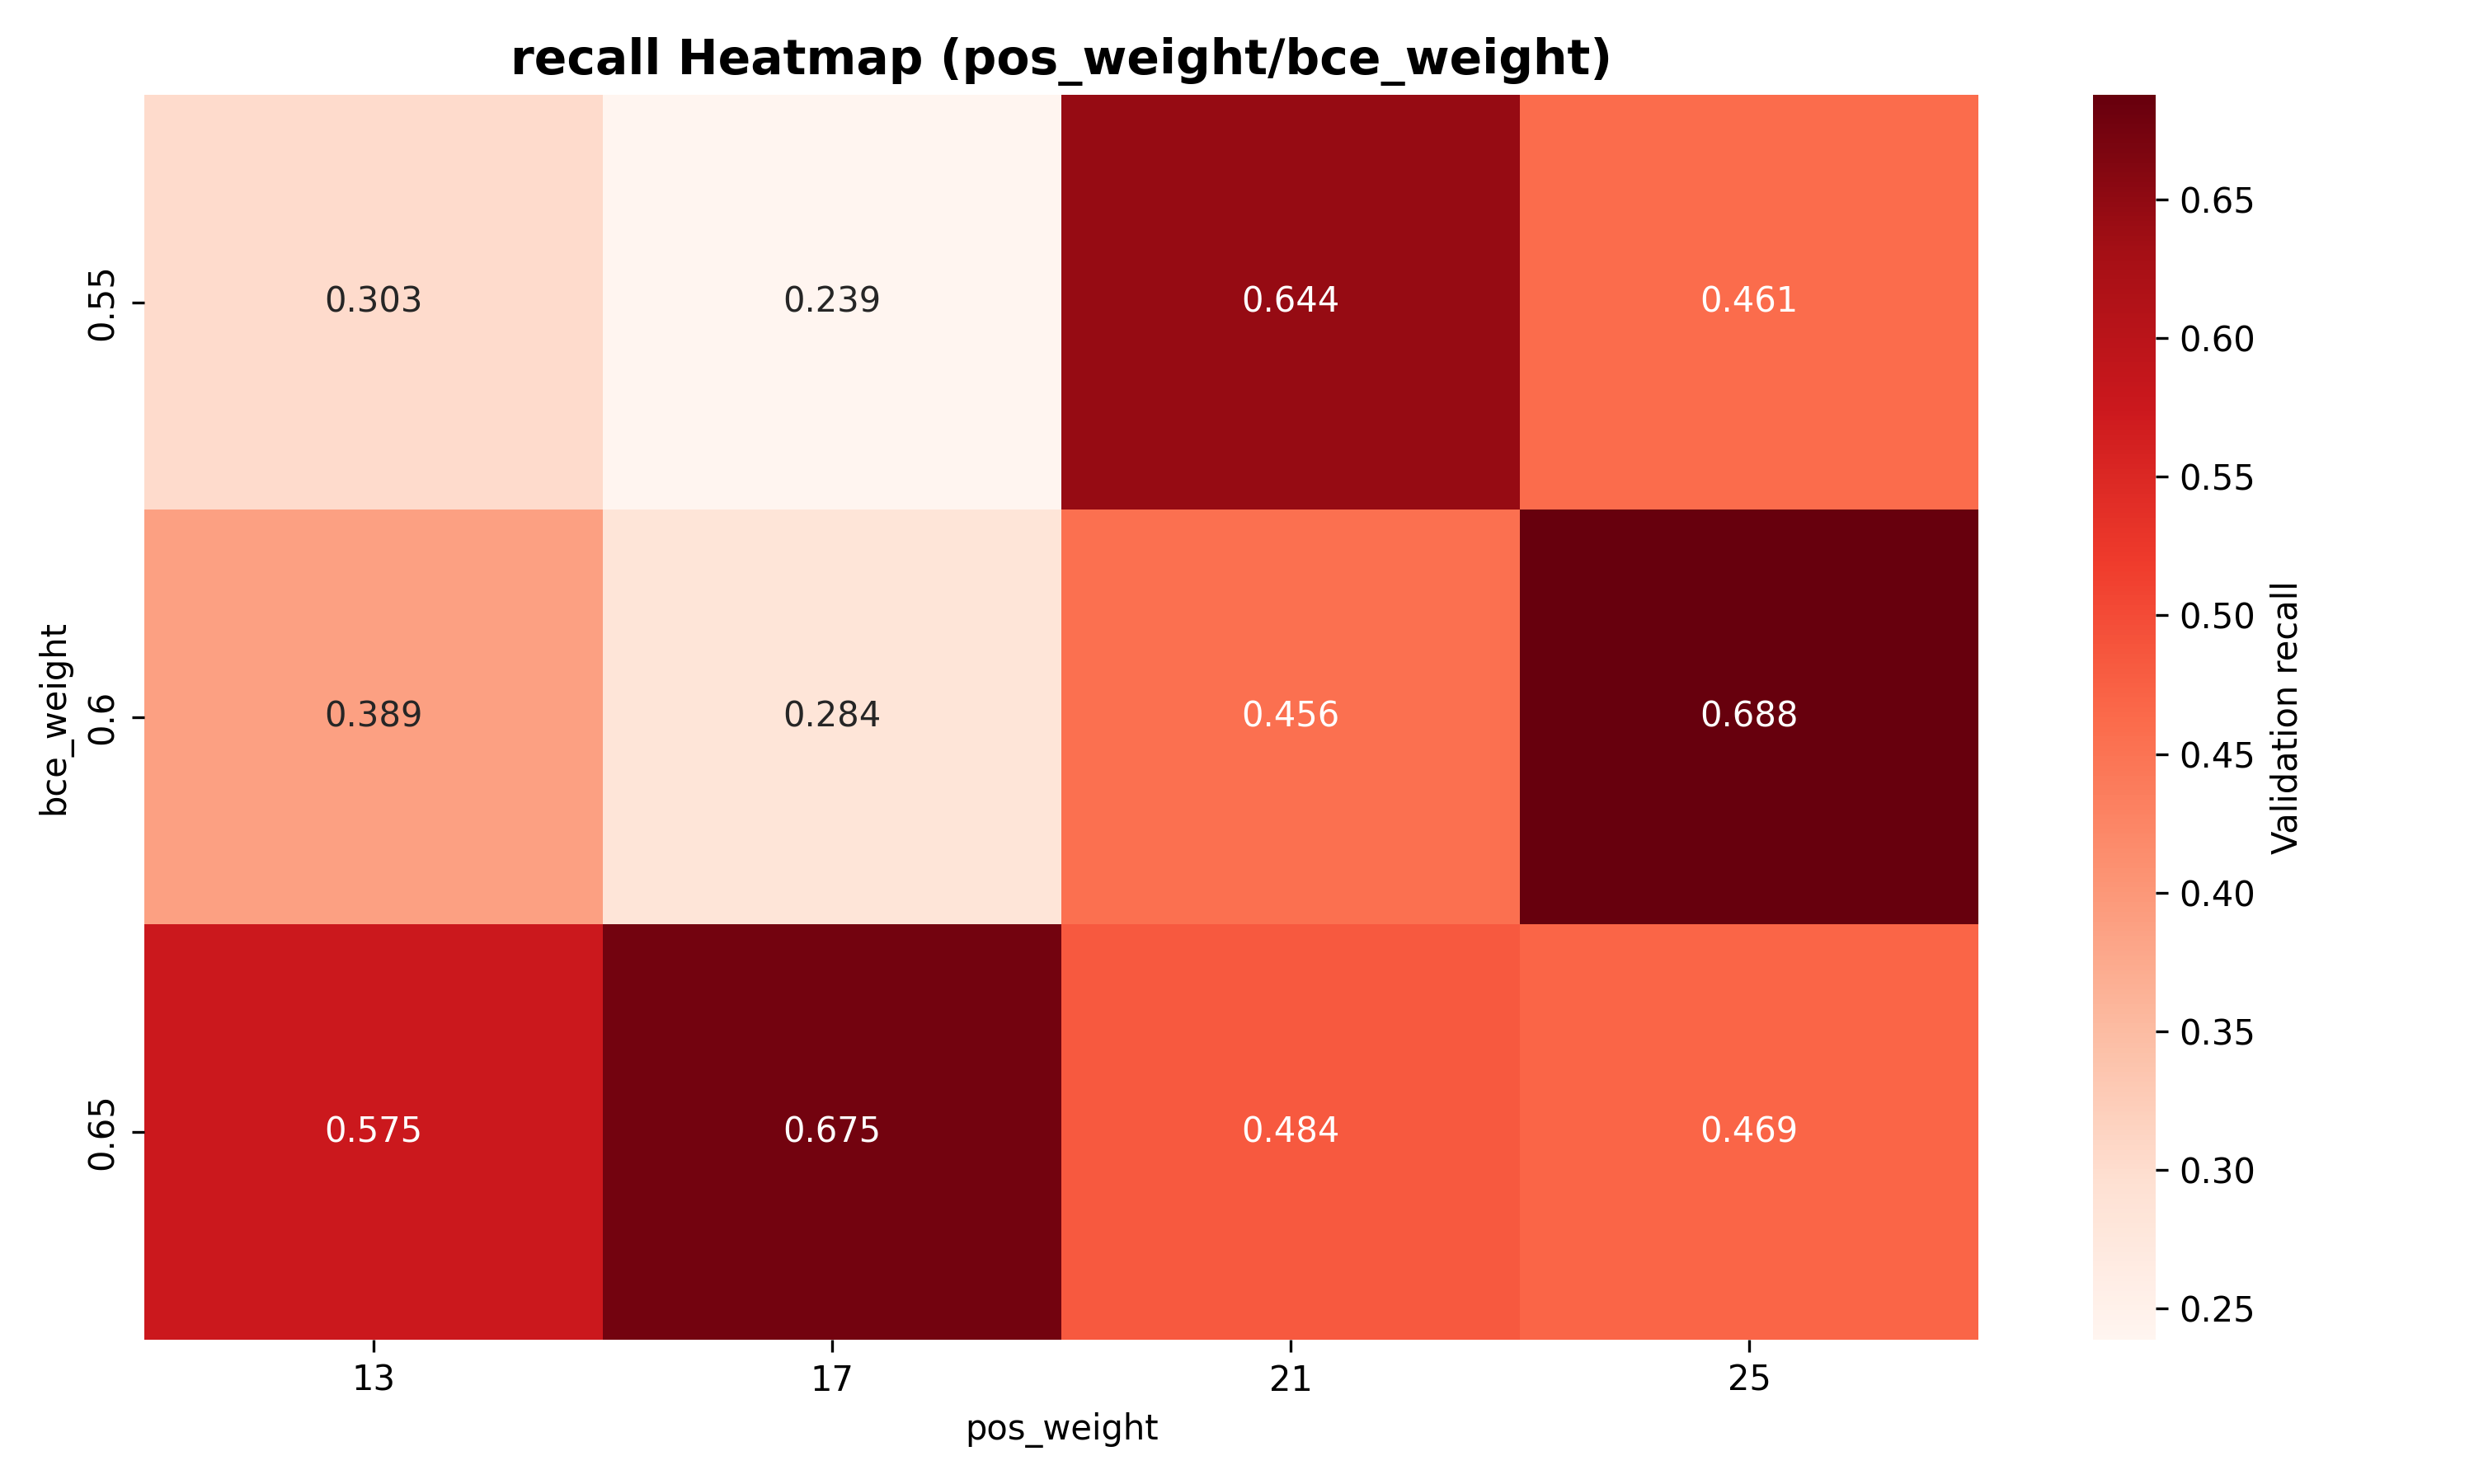
\includegraphics[height=0.7\textheight]{Images/12_heatmap_recall_by_weights.png}
    \end{figure}
\end{frame}

% FlipFlop Graph
\begin{frame}{FlipFlop Graph from Experiment 3}
    \begin{figure}
        \centering
        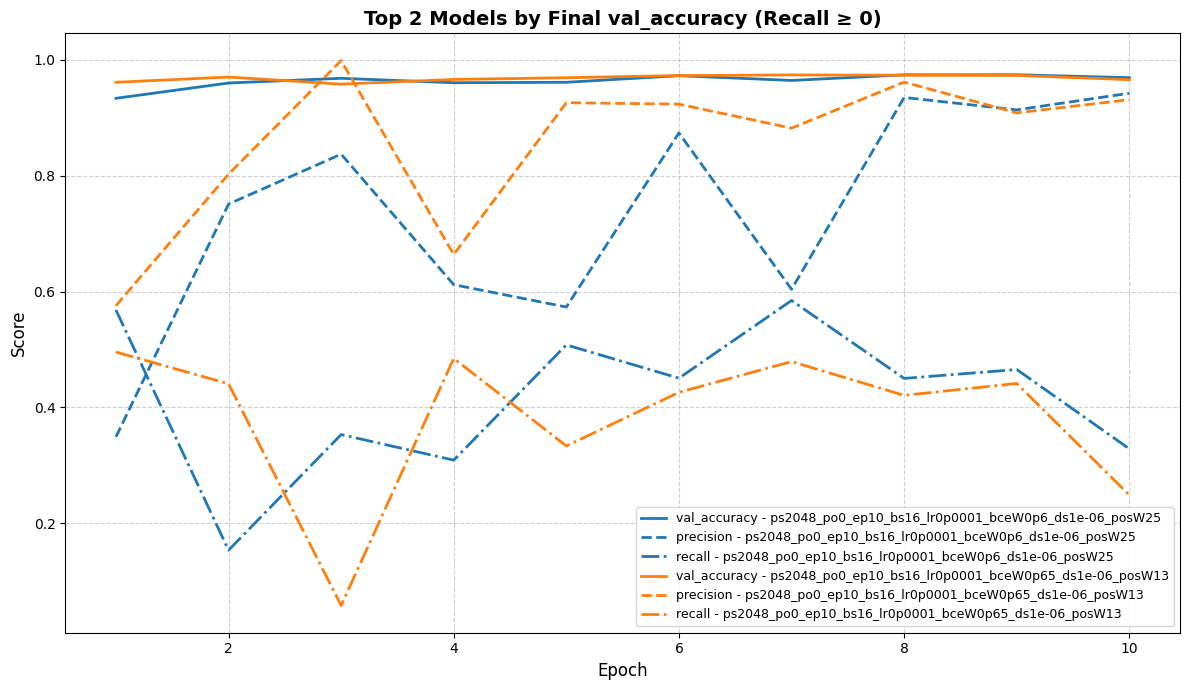
\includegraphics[height=0.7\textheight]{Images/Exp3_acc_prec_rec.png}
    \end{figure}
\end{frame}

\end{document}